\documentclass[a4paper,oneside]{article}
\usepackage{times}
\usepackage{parskip}
\usepackage{tikz}
\usetikzlibrary{calc,shadows,shapes,backgrounds,patterns,arrows,snakes}
\usepackage{graphicx}
\usepackage[pdftex]{hyperref}
\usepackage[section]{placeins}
\pdfadjustspacing=1

\newcommand{\myname}{Radu Hambasan}
\newcommand{\mytitle}{Faceted Search for Mathematics}
\newcommand{\mysupervisor}{Prof. Michael Kohlhase}

\hypersetup{
  pdfauthor = {\myname},
  pdftitle = {\mytitle},
  pdfkeywords = {},
  colorlinks = {true},
  linkcolor = {blue}
}

\bibliographystyle{unsrt}

\usepackage{paralist}
\usepackage{calbf}
\usepackage{lstomdoc}
\lstset{basicstyle=\sf}
\usepackage[show]{ed}

\def\red#1{\textcolor{red}{#1}}
\def\MWS{\textsf{MWS}\xspace}
\def\schemasearch{\textsf{SchemaSearch}\xspace}

\usepackage{wrapfig}
\usepackage{amsfonts}
\usepackage{amsmath}
\usepackage{hyperref}
\newtheorem{definition}{Definition}
\usepackage{xspace}

\usepackage[backend=biber]{biblatex}
\addbibresource{kwarcpubs.bib}
\addbibresource{extpubs.bib}
\addbibresource{kwarccrossrefs.bib}
\addbibresource{extcrossrefs.bib}
\addbibresource{rest.bib}

\usepackage{listings}

\usepackage{bera}
\usepackage{listings}
\usepackage{xcolor}

\colorlet{punct}{red!60!black}
\definecolor{background}{HTML}{EEEEEE}
\definecolor{delim}{RGB}{20,105,176}
\colorlet{numb}{magenta!60!black}
\lstdefinelanguage[m]{MathML}[]{XML}{keywordsprefix={m:},sensitive=true}
\lstdefinelanguage[mws]{MWS}[]{XML}{keywordsprefix={mws:},sensitive=true}
\lstdefinelanguage{json}{
    basicstyle=\normalfont\ttfamily,
    numbers=left,
    numberstyle=\scriptsize,
    stepnumber=1,
    numbersep=8pt,
    showstringspaces=false,
    breaklines=true,
    frame=lines,
    backgroundcolor=\color{background},
    literate=
     *{0}{{{\color{numb}0}}}{1}
      {1}{{{\color{numb}1}}}{1}
      {2}{{{\color{numb}2}}}{1}
      {3}{{{\color{numb}3}}}{1}
      {4}{{{\color{numb}4}}}{1}
      {5}{{{\color{numb}5}}}{1}
      {6}{{{\color{numb}6}}}{1}
      {7}{{{\color{numb}7}}}{1}
      {8}{{{\color{numb}8}}}{1}
      {9}{{{\color{numb}9}}}{1}
      {:}{{{\color{punct}{:}}}}{1}
      {,}{{{\color{punct}{,}}}}{1}
      {\{}{{{\color{delim}{\{}}}}{1}
      {\}}{{{\color{delim}{\}}}}}{1}
      {[}{{{\color{delim}{[}}}}{1}
      {]}{{{\color{delim}{]}}}}{1},
}

\def\cS{\mathcal{S}}
\let\phi=\varphi\let\tilde=\widetilde
\def\mws{\textsf{MathWebSearch}\xspace}
\def\tms{\textsf{TeMaSearch}\xspace}
\def\els{\textsf{Elasticsearch}\xspace}
\def\cmml{\textsf{Content MathML}\xspace}
\def\pmml{\textsf{Presentation MathML}\xspace}
\def\xml{\textsf{XML}\xspace}
\def\xhtml{\textsf{XHTML}\xspace}
\def\xpath{\textsf{XPath}\xspace}
\def\arxiv{\textsf{ArXiv}\xspace}
\def\latexml{\LaTeX{ML}\xspace}
\def\arxmliv{\textsf{ArXMLiv}\xspace}
\def\mathml{\textsf{MathML}\xspace}
\def\zblatt{\textsf{Zentralblatt}\xspace}
\def\latex{\LaTeX\xspace}
\def\tex{\TeX\xspace}

\bibliography{kwarc,rest}

\begin{document}
\pagenumbering{roman}

\thispagestyle{empty}

\begin{flushright}
    
\includegraphics[scale=0.7]{img/jub-logo}
\end{flushright}
\vspace{20mm}
\begin{center}
    \huge
    \textbf{\mytitle}
\end{center}
\vspace*{4mm}
\begin{center}
    \Large by
\end{center}
\vspace*{4mm}
\begin{center}
    \Large
    \textbf{\myname}
\end{center}
\vspace*{20mm}
\begin{center}
    \large
    Bachelor Thesis in Computer Science
\end{center}
\vfill
\begin{flushright}
    \large
    \begin{tabular}{c}
        \mysupervisor \\
        \hline
        Supervisor \\
        \\
    \end{tabular}
\end{flushright}
\vspace*{8mm}
\begin{flushleft}
    \large
    Date of Submission: \today \\
    \rule{\textwidth}{1pt}
\end{flushleft}
\begin{center}
    \Large Jacobs University --- School of Engineering and Science
\end{center}

\newpage
\thispagestyle{empty}

With my signature, I certify that this thesis has been written by me using
only the indicated resources and materials. Where I have presented data and
results, the data and results are complete, genuine, and have been obtained by
me unless otherwise acknowledged; where my results derive from computer
programs, these computer programs have been written by me unless otherwise
acknowledged. I further confirm that this thesis has not been submitted, either
in part or as a whole, for any other academic degree at this or another
institution.

\vspace{20mm}

Radu Hambasan \hfill Bremen, \today

\newpage

\section*{Abstract}
Faceted search represents one of the most practical ways to browse a large
corpus of information. Information is categorized automatically for
a given query and the user is given the opportunity to further refine
his/her query. Many search engines offer a powerful faceted search engine,
but only on the textual level. Faceted Search in the context of Math Search
is still unexplored territory.

In this thesis, I describe one way of solving the faceted search problem in
math: by extracting recognizable formula schemata from a given set of formulae
and using these schemata to divide the initial set into formula classes. Also,
I provide a direct application by integrating this solution with existing
services.

\tableofcontents

\clearpage \pagenumbering{arabic}

\section{Introduction}\label{sec:intro}

The size of digital data has been growing tremendously since the invention
of the Internet. Today, the ability to quickly search for relevant information
in the vast amount of knowledge available is essential in all domains.
As a consequence, search engines have become the prevalent tool for exploring
digital data.

Although text search engines (e.g. Google~\cite{google:online} or
Bing~\cite{bing:online}) seem to be successful for the average user, they are
limited when it comes to finding scientific content. This is because
STEM\footnote{Science, Technology, Engineering and Mathematics} documents are
also relevant for the mathematical formulae they contain and math cannot be
properly indexed by a textual search engine, because the hierarchical structure
of the content is also important.

A good math search engine is therefore needed in several applications.
For example, a large airline manufacturer may have many ongoing research
projects and could significantly improve efficiency if they had a way of
searching for formulae in a corpus containing all their previous work. The same
holds for all large physics-oriented research centers, such as CERN. Valuable
time would be saved if scientists would have a fast, reliable and powerful math
search engine to analyse previous related work. As a third application,
university students should be mentioned. Their homework, research and overall
study process would be facilitated once they are provided with more than
textual search. For all these applications, we need first a strong math search
engine and second a large corpus of math to index.

The Cornell e-Print Archive, \arxiv, is an example of such a corpus, containing
over a million STEM documents from various scientific fields (Physics,
Mathematics, Computer Science, Quantitative Biology, Quantitative Finance and
Statistics)~\cite{arXiv:online}. Having almost a million documents, with
possibly more than a billion formulae, the search engine must provide an
expressive query language and query-refining options to be able to retrieve
useful information. One service that provides both these is the Zentralblatt
Math service~\cite{zbmath:online}.

Zentralblatt Math now employs formula search for access to mathematical
reviews~\cite{KohMihSperTes:mfs13}. Their database contains over 3 million
abstract reviews spanning all areas of mathematics. To explore this database
they provide a powerful search engine called ``structured search''. This engine
is also capable of faceted search.  Figure~\ref{fig:zbFaceted} shows a typical
situation: a user searched for a keyword (here an author name) and the faceted
search generated links for search refinements (the \textbf{facets}) on the
right. Currently, facets for the primary search dimensions are generated --
authors, journals, MSC, but not for formulae. In this way, the user is given
the ability to further explore the result space, without knowing in advance the
specifics of what he/she is looking for.  Recently, formula search has been
added as a component to the structured search facility. However, there is still
no possibility of faceted search on the math content of the documents.

\begin{figure}[ht]\centering
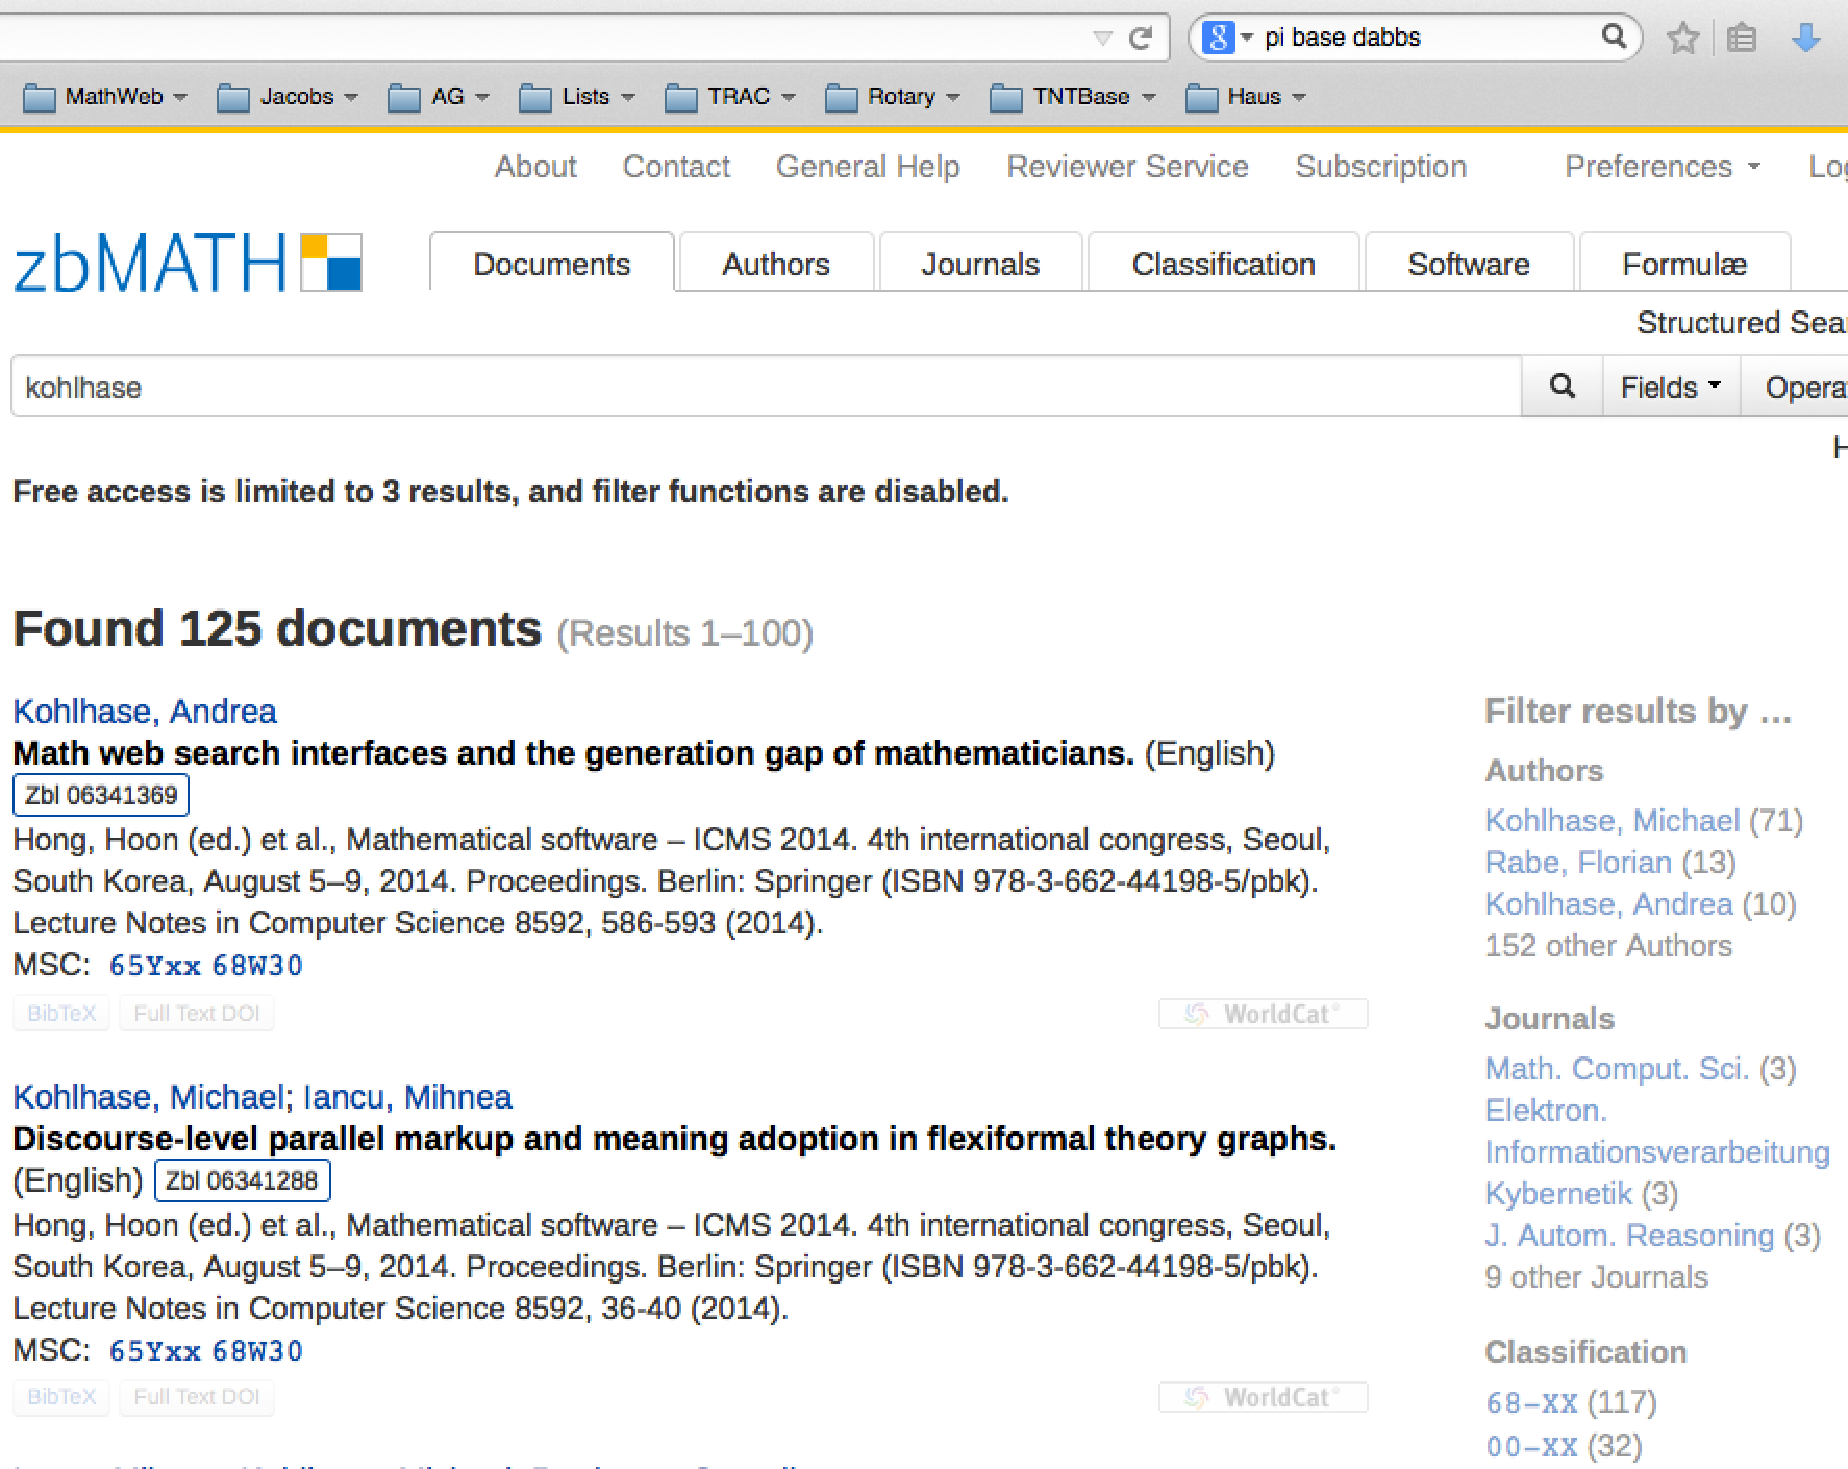
\includegraphics[width=12.1cm]{img/faceted-search.pdf}
\caption{Faceted Search in ZBMath}\label{fig:zbFaceted}
\end{figure}

There are multiple ways in which we could understand a ``math facet''.  One way
would be through the MSC classification~\cite{MSC-SKOS}.  However, this would
be rather vague because it will only provide info about the field of
mathematics to which an article belongs. If the authors use formulae from
another field in their paper, the results will suffer a drop in relevance.

\begin{wrapfigure}r{5.6cm}\vspace*{-1em}
\begin{tabular}{l}
$\int_{\red{M}}{\red\Phi(d_p\red{f}) dvol}$\\[1ex]
$\lambda{\red{X}}.h(H^1\red{X})\cdots{H^n\red{X}}$\\[1ex]
$\frac{\red\Gamma\vdash\red{A}\gg\red\alpha}{\red{D}}$
\end{tabular}\vspace*{-.5em}
\caption{formula facets}\label{fig:formula-facets}\vspace*{-1em}
\end{wrapfigure}

I am attempting to solve this problem by extracting formula schemata from the
query hits as formula facets. A math facet consists of a set of formula
schemata generated to further disambiguate the query by refining it in a new
dimension.  For instance, for the query above we could have the formulae in
Figure~\ref{fig:formula-facets}, which allows the user to drill in on
\begin{inparaenum}[\em i\rm)]
\item variation theory and minimal surfaces,
\item higher-order unification, and
\item type theory.
\end{inparaenum}
Following the \MWS (see~\ref{subsec:prelim:mws}) tradition, the red identifiers
stand for query variables, their presence making the results \textbf{formula
schemata}.

These formula schemata were manually created to judge the feasibility of using
schemata as recognizable user interface entities, but for an application we
need to generate them automatically from the query. Moreover, each schema
should further expand to show the formula class it represents. Formula classes
would consist of all formulae sharing the same schema. This is the algorithmic
problem I explore in the thesis.


\section{Preliminaries}\label{sec:prelim}

In this section we describe the existent systems on which our work will be
based, with the intention of making this thesis self-contained. We will
present these systems in detail in the rest of this section, but
below is a summary of the role they play in our work:
\begin{itemize}
\item \textbf{MathWebSearch} which provides the necessary index structure
for schema search.
\item \textbf{Elasticsearch} which provides hits in response to text query,
    as well as run aggregations on the hits.
    These hits represent formulae to be schematized.
\item \textbf{arXiv} which provides a large corpus of mathematical documents
    that we can index and run our system on.
\item \textbf{\latexml} which converts {\latex} expressions to MathML.
\end{itemize}

\subsection{Project Goals}\label{subsec:prelim:goals}
As discussed in Section~\ref{sec:intro}, the goal of this project is to
develop a scalable formula schematization engine, capable of dividing a set of
query hits into classes, according to the generated formula schemata.

We have set the following end-user requirement for our system:
\begin{enumerate}
    \item[R1.] it should be able to generate formula schemata from a given set
        of formulae and the resulting schemata should be easily recognizable by
        the user.
    \item[R2.] it should be able to classify the given set of formulae
        according to the generated schemata.
    \item[R3.] the system should be massively scalable, i.e. capable of
        answering queries with hundreds of thousands of formulae in a matter of
        seconds.
\end{enumerate}

\subsection{MathWebSearch}\label{subsec:prelim:mws}

At its core, the \mws~\cite{ProKoh:mwsofse11} system (MWS) is a content-based
search engine for mathematical formulae. It indexes MathML~\cite{mathml:online}
formulae, using a technique derived from automated theorem proving:
Substitution Tree Indexing~\cite{Graf94}. Recently, it was augmented with
full-text search capabilities, combining keywords query with unification-based
formula search. The engine serving text queries is
\els~\ref{subsec:prelim:els}.  From now on, in order to avoid confusion, we
will refer to the core system (providing just formula query capability) as \MWS
and to the complete service (\MWS + \els) as \tms (Text + Math Search).

The overall workflow of \tms is the following:
\begin{enumerate}
    \item HTML5 documents representing mathematical articles are
        crawled to generate \MWS harvests~\cite{mwsharvest:online}.
        The \textsf{harvest} format is an extension of \mathml which \MWS can
        index. Its role is to separate the math from the text in a given
        document.
    \item \MWS indexes the harvests.
    \item a second pass is made over the harvests to generate annotated
        documents (see below).
    \item \els indexes the annotated documents.
    \item Everything is now ready for answering queries. When a query is
        issued, \MWS will answer the mathematical part and \els will answer the
        text part.  The results are combined through a
        NodeJS~\cite{nodejs:online} proxy to send a final result set.
\end{enumerate}

Each mathematical expression is encoded as a set of substitutions based
on a depth-first traversal of its \cmml tree.
Furthermore, each tag from the \cmml tree is encoded as a \textsf{TokenID},
to lower the size of the resulting index. The (bijective) mapping is also
stored together with the index and is needed to reconstruct the original
formula. The index itself is an in-memory trie of substitution paths.

For fast retrieval, in the leaves of the substitution tree, \MWS stores
\textsf{FormulaID}s. These are numbers uniquely associated with formulae,
and they are also used to store context and occurrences about the respective
formula. They are stored in a separate LevelDB~\cite{leveldb:online} database.

Figure~\ref{fig:simple_index} shows the core components of \MWS and the
relationship between them. The most important component is the index which
stores the encoded DFS traversal of the formulae from the corpus. This encoding
(from \cmml elements to \textsf{TokenID}s) is handled by the Meaning
Dictionary. As mentioned, each leaf of the index-trie has an associated
\textsf{FormulaID}, which points to the \textsf{FormulaDB}. \textsf{FormulaDB}
includes information about the \xpath and the source documents of every
\textsf{FormulaID}. Finally, there is a \textsf{CrawlDB} database which stores
crawled opaque data, which usually represents the textual part of the source
documents.

\begin{figure}[ht]\centering
    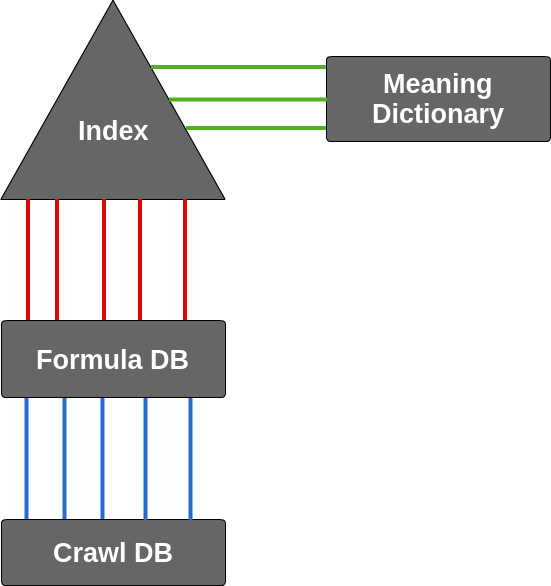
\includegraphics[scale=0.3]{img/simple_index.png}
    \caption{MWS core components}\label{fig:simple_index}
\end{figure}
\FloatBarrier

\mws exposes a RESTful HTTP API which accepts \xml queries.
A valid query must obey the \cmml format, potentially augmented with
\emph{qvar} variables which match any subterms.  A \emph{qvar} variable acts as
a wildcard in a query, with the restriction that if two \emph{qvar}s have the
same name, they must be substituted in the same way.

\tms is using both \mws and \els to answer queries.
In order to achieve cooperation between the two systems, annotated documents
are used. These annotated documents contain metadata from the original document
(e.g. URI, title, author, etc.) and a list of \textsf{FormulaID}s that can be
found in that document.

\subsection{Elasticsearch}\label{subsec:prelim:els}
Elasticsearch~\cite{esl:online} is a powerful and efficient full text search
and analytics engine, built on top of Lucene. It can scale massively, because
it partitions data in shards and is also fault tolerant, because it replicates
data.  It indexes schema-free JSON documents and the search engine exposes a
RESTful web interface.  The query is also structured as JSON and supports a
multitude of features via its domain specific language:  nested queries,
filters, ranking, scoring, searching using wildcards/ranges and faceted search.

The faceted search feature\footnote{Faceted search as such is now deprecated in
    ES and was replaced by the more powerful ``aggregations'' feature, which
    also allows facets of facets, i.e. nested facets.} is of
particular interest to us. 
One way to use this feature is the terms aggregation: a multi-bucket
aggregation, with dynamically built buckets.  We can specify an array field
from a document and ask ES to count how many unique items from the array are
there in the whole index.  This list can also be sorted, e.g. most frequently
occurring items first.  Additionally, we can also impose a limit on the number
of the buckets (items) for which we want to receive the count.

An ES query which would return the most frequently used formulae (and
subformulae) for ``Pierre Fermat'', is presented in
Listing~\ref{lst:es_agg_query}. The key part is the \emph{aggs} fields. We are
specifying that we want an aggregation called \textit{Formulae} on ``terms''
(i.e. we want bucket counting) and the target of the aggregation is the fields
\emph{ids}.

\begin{lstlisting}[language=json,firstnumber=1,caption=Elastic Search Term
Aggregation Query, captionpos=b, label=lst:es_agg_query]
{
  "query" : {
      "match" : {
          "body" : {
              "query" : "Pierre Fermat",
              "operator" : "and"
          }
      }
  },
  "aggs" : {
      "formulae" : {
          "terms" : { "field" : "ids" }
      }
  }
}
\end{lstlisting}

A possible response to the above query can be found in
Listing~\ref{lst:es_agg_resp}. In the response we can see the returned
aggregations. In our example there is only one and it is called
\emph{formulae}. We can find the actual result in the \emph{buckets} field. The
\textsf{key} field in the bucket corresponds to a \textsf{FormulaID}.
Here, the most frequent formulae were the one with ID 230 and the one with ID
93. The former appeared in 10 documents and the latter appeared in 9 documents.

\begin{lstlisting}[language=json,firstnumber=1,caption=Elastic Search Term
Aggregation Response, captionpos=b, label=lst:es_agg_resp]
{
    ...
    "aggregations" : {
        "formulae" : {
            "buckets" : [
                {
                    "key" : "230",
                    "doc_count" : 10
                },
                {
                    "key" : "93",
                    "doc_count" : 9
                },
                ...
            ]
        }
    }
}
\end{lstlisting}

\subsection{arXiv}\label{subsec:arxiv}
\textbf{arXiv} is a repository of over one million publicly accessible
scientific papers in STEM fields. For the NTCIR-11
challenge~\cite{HamKohPro:man14},
MWS indexed over 8.3 million paragraphs (totaling 176 GB) from arXiv. We will
base our queries on this large index, because it provides a rich database of
highly relevant formulae. Moreover, Elasticsearch will have more formulae on
which it can run aggregations, also leading to more relevant results.

\subsection{\latexml}\label{subsec:latexml}
An overwhelming majority of the digital scientific content is written using
\latex or \tex, due to its usability and popularity among STEM researchers.
However, formulae in these formats are not good candidates for searching
because they do not display the mathematical structure of the underlying
idea. For this purpose, conversion engines have been developed to convert
\latex expressions to more organized formats such as \mathml.

An open source example of such a conversion engine is
\latexml~\cite{Miller:latexml:online}. The \mws project relies heavily on it,
to convert \arxiv documents from \latex to XHTML which is later indexed by \MWS.
It exposes a powerful API, allowing definition files to relate \tex elements to
corresponding XML fragments that should be generated.
For the scope of this project, we will be more interested in another feature of
\latexml: cross-referencing between \pmml and \cmml. While converting \tex
entities to a \pmml tree, each element receives a unique identifier which is
later referenced from the corresponding \cmml element. In this manner, we can
modify the \cmml tree and reflect the changes in the \pmml tree which can be
displayed to the user.

Figure~\ref{fig:crossreference_diag} illustrates the parallel markup for
$\frac{2}{x+3}$. On the left side we have \pmml and on the right side, \cmml.
As we can see, every Presentation element has a Content correspondent, except
the \textsf{divide} operator.

\begin{figure}[ht]\centering
    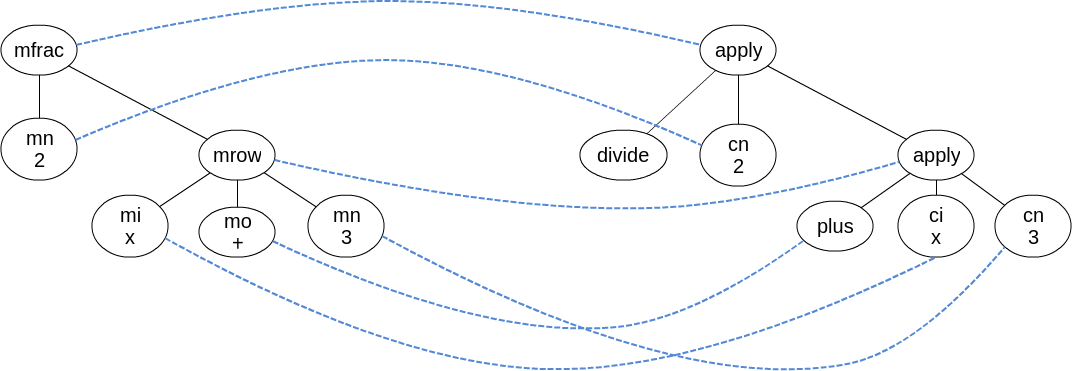
\includegraphics[scale=0.3]{img/crossreference_diag.png}
    \caption{The CMML/PMML parallel markup}\label{fig:crossreference_diag}
\end{figure}
\FloatBarrier


\section{Implementation}\label{sec:implementation}

In this section, I explain the key details of the formula classifier's
implementation, the overall system architecture, as well as the challenges and
trade-offs associated with the taken design decisions.

\subsection{Formalizing the problem}\label{subsec:formal_problem}
Let us now formulate the problem at hand more carefully.

\begin{definition}
  Given a set $\cD$ of documents (fragments) -- e.g. generated by a search
  query, a \textbf{coverage} $0<r\leq1$, and a \textbf{width} $n$, the
  \textbf{Formula Schemata Generation} (FSG) problem requires generating
  a set $\cF$ of at most $n$ formula schemata (content MathML expressions with
  \lstinline|qvar| elements for query variables), such that $\cF$ covers $\cD$
  with coverage $r$.
\end{definition}

\begin{definition}
  We say that a set $\cF$ of formula schemata \textbf{covers} a set $\cD$ of
  document fragments, with \textbf{coverage} $r$, iff at least $r \cdot |\cD|$
  formulae from $\cD$ are an instance $\sigma(f)$ of some $f\in\cF$ for a
  substitution $\sigma$.
\end{definition}

\subsection{An Algorithm for FSG}\label{subsec:fsgAlgorithm}
I present an FSG algorithm and its implementation. It requires a \MWS index of
the corpus. Given such an index, and a set $\cD$ of formulae (as CMML
expressions), we can find the set $\cF$ in the following way:
\begin{enumerate}
    \item Parse the given CMML expressions similarly to \MWS queries,
        to obtain their encoded DFS representations.
    \item Choose a reasonable cutoff heuristic, see~\ref{subsec:cutoffheur}.
    \item Unify each expression with the index, up to a given threshold (given
        by the above heuristic).
    \item Keep a counter for every index path associated with the unifications.
        Since we only match up to a threshold, some formulae will be associated
        with the same path (excluding the leaves).
        We increase the counter each time we find a path already associated
        with a counter.
    \item We sort these path-counter pairs by counter in descending order and
        take the first $n$ ($n$ being the width required by the FSG).
    \item If the threshold depth was smaller than a formula's expression
        depth, the path associated with it will have missing components. We
        replace the missing components with \lstinline|qvar|s to generate the
        schema and return the result set.
\end{enumerate}

\begin{wrapfigure}r{5.6cm}\vspace*{-1em}
    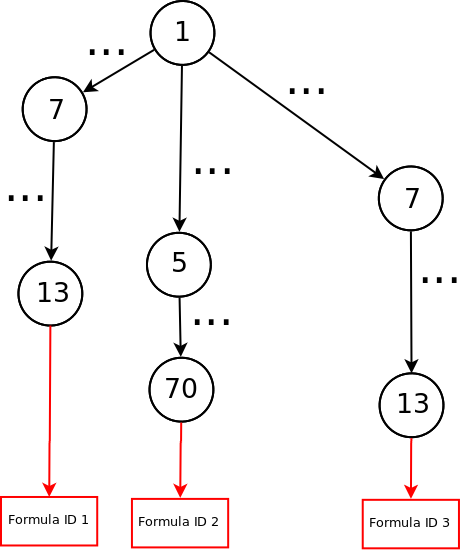
\includegraphics[scale=0.24]{img/FFG_Algo_diag.png}
\caption{Simplified index at depth 1}\label{fig:algoindex}
\end{wrapfigure}

Figure~\ref{fig:algoindex} shows a simplified \MWS index at depth 1.
The formulae's paths represent their depth-first traversal.
Every formula can be reconstructed given its path in the index.
The circles represent index nodes and the number inside represents
the token's ID. When we reach a leaf node, we completely described a
formula. This is encoded in the leaf node by an ID, which can be used
to retrieve the formula from the database.
The length of the arrows symbolizes the depth of the omitted subterms
(for higher depths, we have longer arrows).
Notice how both formula with ID 1 and formula with ID 3 show the same
``path'' when ignoring subterms below a cutoff depth.

\subsection{Finding a cutoff heuristic}\label{subsec:cutoffheur}
To generate formula schemata, we must define a ``cutoff heuristic'',
which tells the program when two formulae belong to the same schema class.
If there is no heuristic, two formulae would belong to the same class,
only if they were identical. However, we want formulae that have something in
common to be grouped together, even if they are not perfectly identical.

\subsubsection{Absolute cutoff}\label{subsubsec:absolute_cutoff}
One reasonable cutoff heuristic would be a fixed expression depth, given as a
parameter to the Schematizer. In this way, a depth of 0 would always return
$?x$ which corresponds to the 0-unification.
Figure~\ref{fig:cutoff_naive} illustrates the absolute cutoff heuristic.
On the left side, we have the initial \cmml representation for the formula
$\frac{2}{x+3}$. Using an absolute cutoff depth of 1, we get the CMML
representation of the schema shown on the right side.

\begin{figure}[ht]\centering
    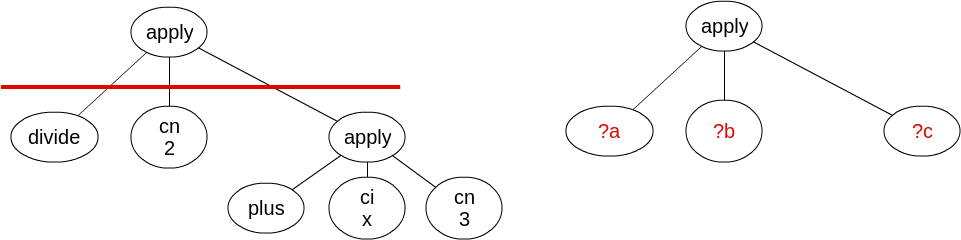
\includegraphics[scale=0.3]{img/cutoff_naive.png}
    \caption{Cutoff at a fixed depth}\label{fig:cutoff_naive}
\end{figure}
\FloatBarrier

Using this heuristic, we are able to group together formulae which share a
certain portion of their \cmml representation and return this shared portion as
the group's schema. However, in practice this approach poses several
disadvantages. By using a uniform cutoff for a given CMML tree, we might also
remove the operator of an expression (first child of the \textsf{apply} node).
This leads to unintuitive instantiations from the user point of view. For
example, the schema $\red{?x} + \red{?y}$ will also include $a - b$ in its
class, which is not desired since we only want to abstract out the operands of
an expression.

\subsubsection{Relative cutoff}\label{subsubsec:relative_cutoff}
A slight improvement over the absolute cutoff heuristic would be to choose the
cutoff depth depending on the depth of the CMML tree. For this, the user would
specify a relative cutoff, e.g. $50\%$, and each tree would be truncated at
that relative depth.

On an individual basis, we are still using a uniform cutoff, so this approach
also poses all disadvantages outlined in the previous section. The main
advantage of this method stems from the ability to differentiate between
complex and trivial formulae. If the cutoff were absolute, for low depths,
complex formulae would be truncated into simple schema. This would mean that
the user has the choice to either see only the simple schemata, or only the
complex ones. By using the relative heuristic, both complex and simple schemata
would share the result set.

\subsubsection{Dynamic cutoff}\label{subsubsec:dynamic_cutoff}
As we have already seen, a uniform cutoff heuristic is generally not the
optimal choice as it also removes operators. We would like to ``schematize''an
expression by abstracting out only the operands, while leaving the operators
untouched. To do this, we can completely expand the first child of an
\textsf{apply} tag and apply the cutoff depth (either absolute or relative)
only to the other nodes. Figure~\ref{fig:cutoff_dynamic} illustrates this
heuristic at depth 1. The \textsf{divide} element was kept, because it was the
first child of \textsf{apply}, while the other children were removed.
If we were to use a depth of 2, the \textsf{plus} element would also be
included in the schema.

\begin{figure}[ht]\centering
    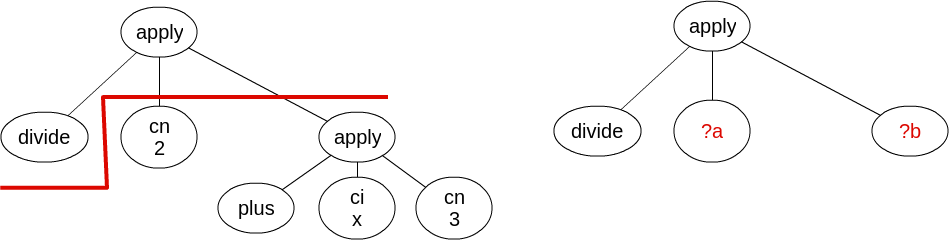
\includegraphics[scale=0.3]{img/cutoff_dynamic.png}
    \caption{Dynamic cutoff}\label{fig:cutoff_dynamic}
\end{figure}
\FloatBarrier

Although this method seems to yield recognizable schemata and classes with
intuitive instantiations, it is relatively difficult to implement because the
operator might occupy several levels (not just one, as shown in the figure) and
we must do the expansion directly using the DFS traversal of the CMML tree.

\subsubsection{Coverage-aware cutoff}\label{subsubsec:coverage_aware_cutoff}
To report optimal results to the user, we could try a ``brute-force'' approach,
in which we compute the schematization for a large range of fixed depths, and
then select schemata with the \textit{best} coverage from all the results. The
best coverage should not be too large (because this could mean it is a trivial
schema) and also not too small (because this could mean the schema is not
important). Consequently, we will choose several cutoffs for a given query.
However, this method is very computationally expensive and defeats
the \textsf{R3} goal of this project.

\subsubsection{Length based cutoff}\label{subsubsec:length_based_cutoff}
Another possibility is to place the cutoff on length, instead of depth. This
method would group together formulae which begin the same way. To implement
a length based cutoff, we generate the DFS encoding of a formula and then take
the first $n$ tokens, where $n$ is a given cutoff. Despite being relatively
easy to implement and fast to compute, this heuristic would generate results
which are not as interesting as those generated by a depth based heuristic
(because the former will only show the first few elements in a formula, whereas
the latter will also show the last tokens).

\subsubsection{Combining heuristics}\label{subsubsec:combining_cutoffs}
As we have seen, there are several advantages and drawbacks associated with
each heuristic. Since the coverage-aware cutoff is too expensive to compute and
the length-based cutoff does not generate interesting enough results, we
will ignore them when proposing the following combined heuristic. In our
project we use the dynamic cutoff (thus preserving operators) and offer the
user a choice on whether the operands cutoff should be absolute or relative.


\subsection{Design Overview}\label{subsec:design_overview}
\begin{wrapfigure}r{5.6cm}\vspace*{-1em}
    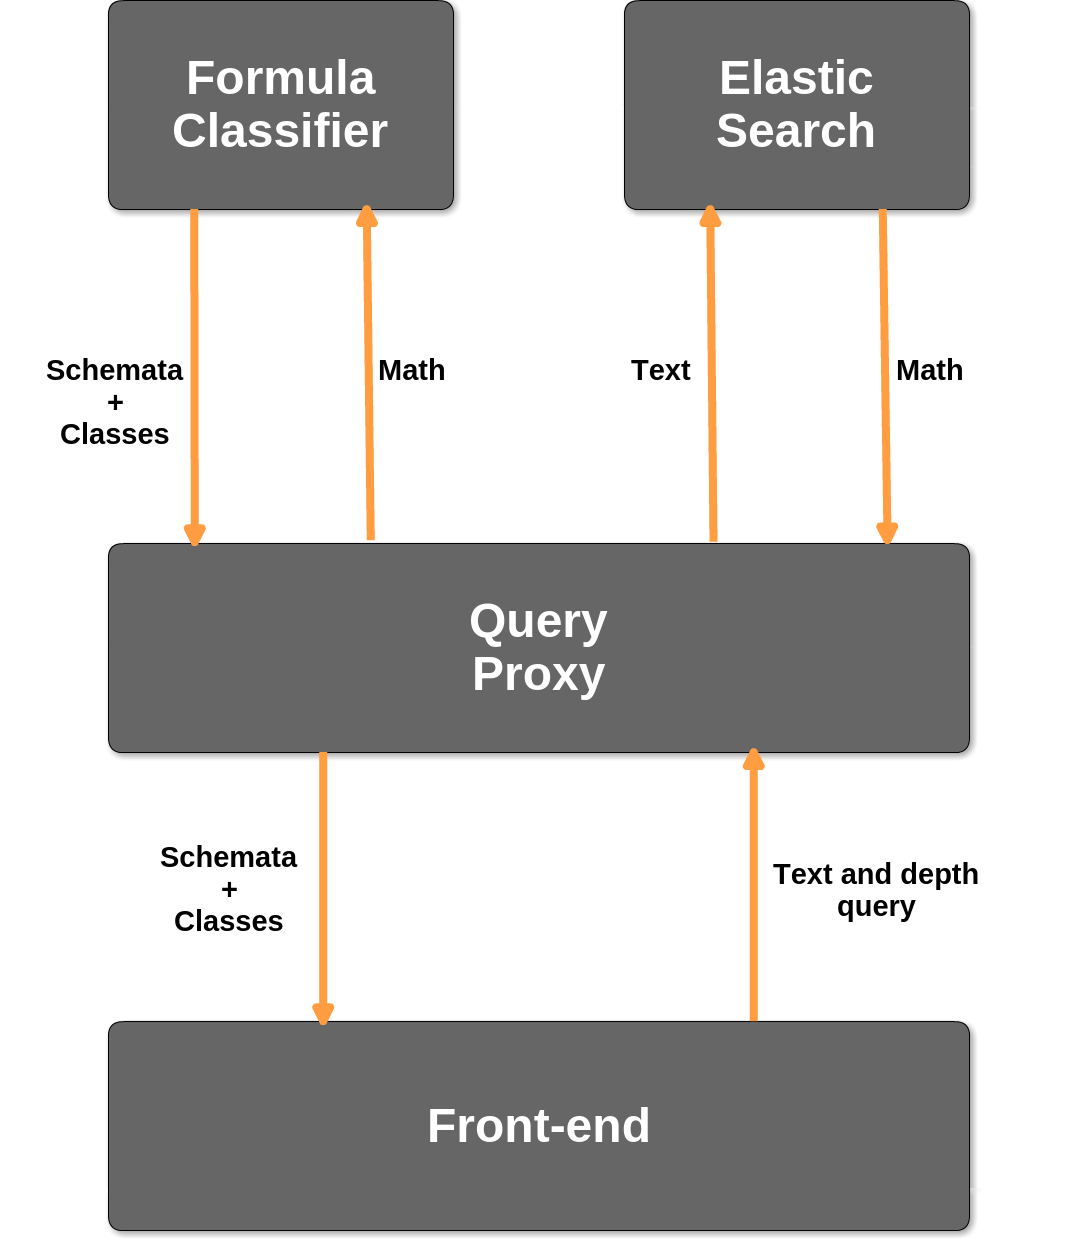
\includegraphics[scale=0.15]{img/SchemaArchitecture.png}
    \caption{FS engine architecture}\label{fig:sys_architecture}
\end{wrapfigure}

The full faceted search system comprises of the following components: the
Formula Schematizer~\ref{subsec:fschematizer}, Elasticsearch, a proxy to
mediate communication between the Schematizer and Elasticsearch and a Web
front-end. The architecture of the system is shown in
Figure~\ref{fig:sys_architecture}. 

Once the user enters a query (which consists of keywords and a depth), the
front-end forwards the request to a back-end proxy. The proxy sends the
text component of the query to Elasticsearch and receives back math
contained in matching documents. Afterwards, it sends the retrieved math
and the depth (from the original query) to the Schematizer. The Schematizer
will respond with a classification of the math in formula classes, as well
as the corresponding schema for each class. Finally, the proxy forwards the
result to the front-end which displays it to the user.

In the following sections, I will explain the core components of
the system in detail and describe the challenges faced during
implementation.

\subsection{The Formula Schematizer}\label{subsec:fschematizer}
The Schematizer is the central part of our system. It receives a set of
formulae in their \cmml representation, generates corresponding formula
schemata and classifies the formulae according to the generated schemata.
It provides an HTTP endpoint and is therefore self-contained, i.e. it can be
queried independently, not only as part of the faceted search system.
As a consequence, the Schematizer displays a high degree of versatility,
and can be integrated seamlessly with other applications.

Although the algorithm described in Section~\ref{subsec:fsgAlgorithm} works
well in theory, we needed to adapt it considering various \mws implementation
details, e.g. the index is read-only (therefore we cannot store extra data into
the index nodes). Therefore, the overall idea/theory is the same, but now we
take the following shortcut: instead of unifying every formula with the index,
we just pretend we do and instead generate a ``signature'' for each formula.
This signature is the path shown in Section~\ref{subsec:fsgAlgorithm}. We use
the \mws encoding for \mathml nodes, where each node is assigned an integer ID
based on its tag and text content. If the node is not a leaf, then only the tag
is considered. The signature will be a vector of integer IDs, corresponding to
the pre-order traversal of the \cmml tree.

Naturally, the signature depends on the depth chosen for the cutoff heuristic.
At depth 0, the signature consists only of the root token of the \cmml
expression. At full depth (the maximum depth of the expression), the signature
is the same as the depth-first traversal of the \cmml tree.

Based on these computed signatures, we divide the input set of formulae into
formula classes, i.e. all formulae with the same signature belong to the same
class. For this operation we keep an in-memory hash table, where the keys are
given by the signatures and the values are sets of formulae which have the
signature key. After filling the hash table, we sort it according to the number
of formulae in a given class, since the signatures which cover the most
formulae should come at the beginning of the reported result.

The Schematizer caller can place a limit on the maximum number of schemata to
be returned. If such a limit was specified, we apply it to our sorted list of
signatures and take only the top ones.

As a last step, we need to construct \cmml trees from the signatures,
to be able to show the schemata as formulae to the user. We are able to do
this because we know the arity of each token and the depth used for cutoff.
The tree obtained after the reconstruction might be incomplete, so we insert
query variables in place of missing subtrees.
We finally return these \cmml trees with query variables (the formula
schemata), together with the formulae which they cover.

\subsection{The Elasticsearch proxy}\label{subsec:esproxy}
To obtain formulae to feed as input to the Schematizer, we make use of
Elasticsearch. The corpus indexed by Elasticsearch consists of 176 GB of \arxiv
documents annotated using the format described in
Section~\ref{subsec:prelim:mws}.

To mediate the communication between the two components (Elasticsearch and the
Schematizer), a NodeJS proxy was developed. The proxy exposes an HTTP
interface, which will be used by an eventual front-end for querying.
There are three important query parameters: the keywords, the depth and the
maximum schemata count.

The main task of the proxy is to assemble the Elasticsearch JSON query after
receiving the parameters from the front-end and forward the Elasticsearch
results to the Schematizer. To ensure a fast response, only a minimum of
preprocessing is done between the stages.

Once the Schematizer has generated schemata and has classified the formulae,
the proxy assembles the results into a JSON object which it sends to the
front-end.

\subsection{The Front-End}\label{subsec:frontend_schema}
To show the capabilities of the Schematizer we have prepared two demos.
The first one is a text-only search engine which returns the math from the
matching documents, after running it through the Schematizer. This is the demo
for showcasing the schematization process. The second one is a direct
application of the Schematizer into a Math Search Engine which is capable of
mathematical faceted search.

\subsubsection{SchemaSearch}
The \textsf{SchemaSearch} front-end provides just a textual search input field.
It is intended for users who want an overview of the formulae contained in a
corpus.
As shown in figure~\ref{fig:frontend_schema}, the user can enter a set of
keywords for the query, as well as a schema depth, which defaults to 3. The
maximum result size is not accessible to the user, to prevent abuses and reduce
server load.  There is also an ``R'' checkbox which specifies if the cutoff
depth should be absolute or relative. If relative, the depth should be given in
percentages.

\begin{figure}[ht]\centering
    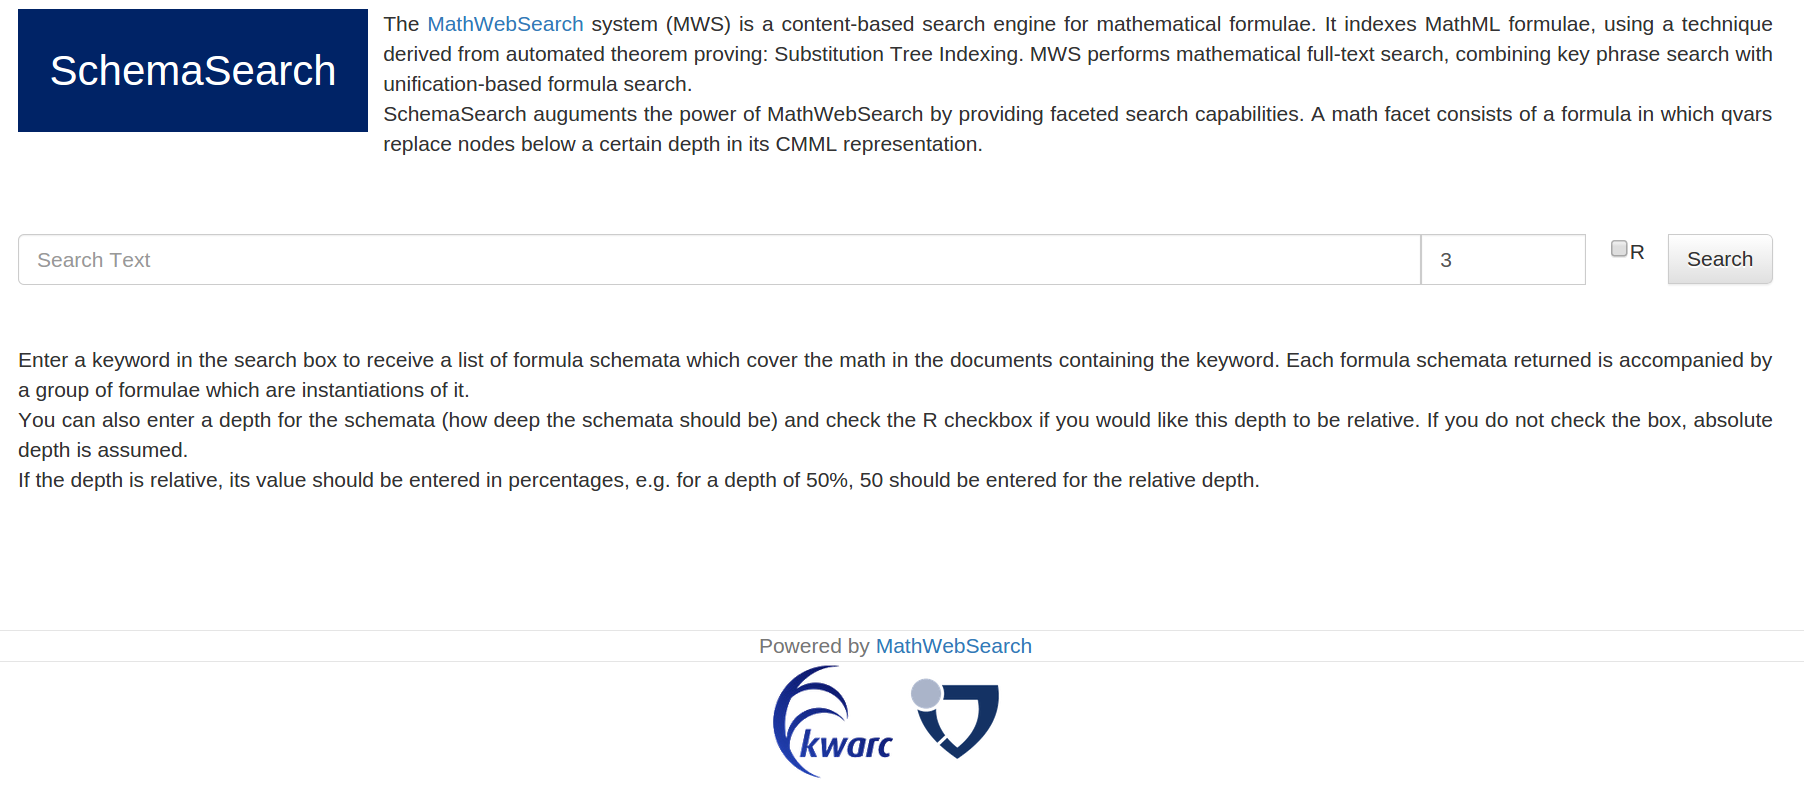
\includegraphics[width=12.1cm]{img/frontend_schema.png}
    \caption{SchemaSearch front-end}\label{fig:frontend_schema}
\end{figure}
\FloatBarrier

\subsubsection{TemaV2}
The \textsf{TemaV2} front-end extends \tms to be able to perform mathematical
faceted search. It is intended for users who want to filter query results based
on a given facet (formula schema in this case).
The look and feel is similar to the previous version of \tms,
as shown in Figure~\ref{fig:frontend_temaV2}, where the first input field is
used to specify keywords and the second one is used to specify \latex-style
formulae for the query. When returning results, a ``Math Facets'' menu will be
presented to the user. We discuss this in
Section~\ref{subsec:fe_results_display2}.

\begin{figure}[ht]\centering
    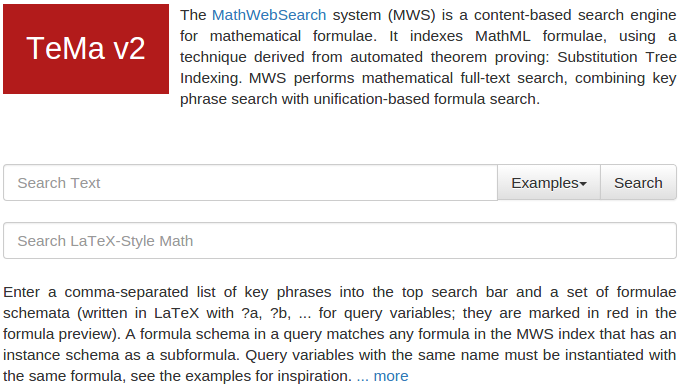
\includegraphics[width=12.1cm]{img/frontend_temaV2.png}
    \caption{TemaV2 front-end}\label{fig:frontend_temaV2}
\end{figure}
\FloatBarrier

\subsection{ES aggregations}\label{subsec:esagg}
Initially, the ``aggregations'' feature of Elasticsearch seemed to be a
suitable improvement for the Schematizer and the ES script was originally
designed to request math in a term-based aggregation format, as described in
Section~\ref{subsec:prelim:els}. However, on a closer look we can see that not
only are aggregations not needed, but they influence the results in a negative
way.

On a regular query, the top formulae reported using aggregations were trivial
formulae, i.e. consisting of only one or two symbols. This is because authors
frequently use short inline math to refer to their results. As a consequence,
the top returned was completely unusable, because the first hits were
irrelevant. Moreover, it was impossible to distinguish between long irrelevant
expressions and infrequently used important expressions since both of them
ranked the same.

As an added disadvantage of using aggregations, we must mention the time
overhead. For obtaining accurate results over the entire index, several minutes
were needed. In order to reach our target time of $\approx 10s$, we had to
drastically shrink down the number of considered aggregations (down to 100).
As mentioned before, all these 100 expressions were trivial.

Given the drawbacks mentioned above, we decided against using aggregations in
the Schematizer pipeline. As an alternative, we will retrieve all math content
from the documents which match the keywords and discard the trivial formulae
using a configurable length heuristic. In practice, this change allowed us to
process more than ten thousand formulae in less than five seconds, which is a
drastic improvement from the approach using aggregations.

\subsection{Presentation by replacement}\label{subsec:make_sch_recog}
After obtaining the schemata and formula classes, we need to be able to display
the result to the user. One possibility would be to have the Schematizer return
\cmml expressions for the schemata and use an XSL
stylesheet~\cite{carlisle:online} to convert them to \pmml. This approach
would unfortunately generate unrecognizable schemata due to the inherent
ambiguity of CMML. For instance, a \textsf{csymbol} element can be
represented in several different ways depending on the notation being used.
Additionally, we cannot reliably foresee all possible rules that should be
implemented in the stylesheet and as a consequence some formulae will be
wrongly converted.

Since the XSL conversion is unreliable, we will make use of the cross-reference
system provided by \latexml, as discussed in Section~\ref{subsec:latexml}.
Instead of returning \cmml expressions, the Schematizer will use the first
formula in each class as a template and ``punch holes into it'', effectively
returning the ID of the nodes that are to be substituted with query variables.
We will use this IDs to replace the referenced PMML nodes with \verb|<mi>|
nodes representing the qvars.

Figure~\ref{fig:replacement_pres} shows the presentation by replacement
technique for a given schema. The Schematizer returned a schema which was
checked against the first formula in its class ($\frac{2}{x+3}$) to generate
two substitutions, marked with red on the left side. Due to the cross-reference
system provided by \latexml, we are able to find the corresponding PMML
elements and substitute them with \verb|<mi>| tokens.

\begin{figure}[ht]\centering
    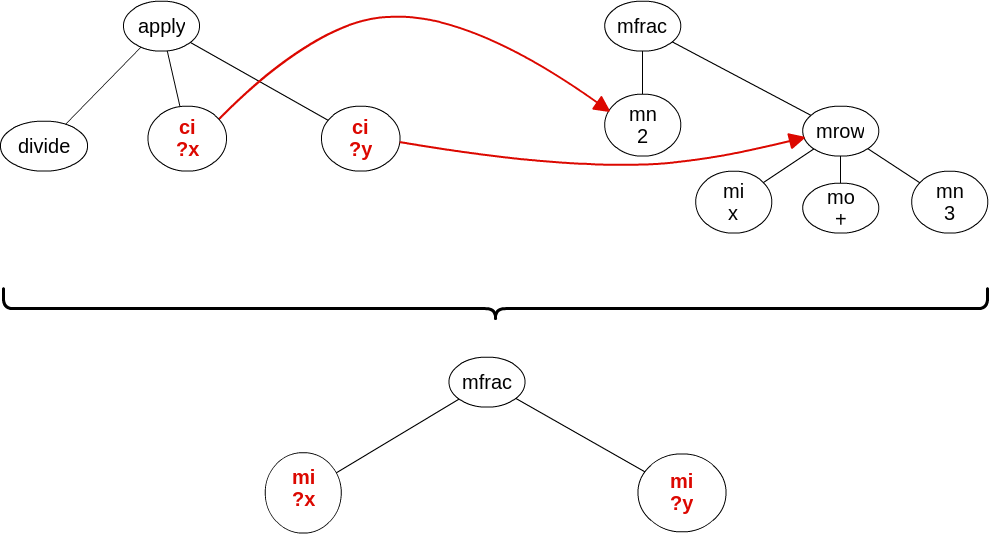
\includegraphics[scale=0.3]{img/replacement_pres.png}
    \caption{Presentation by replacement}\label{fig:replacement_pres}
\end{figure}
\FloatBarrier

\subsection{Naming query variables}\label{subsec:naming_qvars}
As discussed in the section before, we will need a template to modify in order
to display the schema of a class. We are using the first formula as a template,
but any formula in a given class would work as a template for that class.
Since we will process an existing expression, it would be appropriate to name
the query variables in a way which allows the user to perceive some meaning
behind them. For this reason, we conceived a naming convention with the
following rules:

\begin{itemize}
    \item If the node to be replaced is a leaf, its name will be used for the
        qvar.
    \item If the node to be replaced is not a leaf (thus having no name), we
        will use lowercase alphabetical letters from \textsf{a} to \textsf{z}
        preceded by a question mark (according to the \MWS tradition).
    \item If there are more than 26 qvars (thus exceeding the alphabet), we
        name them $x_{1}, x_{2}, \ldots, x_{max\_count}$, also preceded by a
        question mark. This case should be extremely rare.
\end{itemize}

\section{Evaluation}\label{sec:evaluation}

In this section, we will present an evaluation of our faceted search engine.
Firstly, we will examine the 2 front-ends, obtained after applying the
heuristics and improvements described in the Implementation section. Next, we
will analyze the performance of the Schematizer deployed on an \arxiv index
(\ref{subsec:sch_performance}). In the end, we will look at the API that the
Schematizer exposes and elaborate on its potential
(\ref{subsec:schematizer_api}).

\subsection{SchemaSearch front-end}\label{subsec:fe_results_display1}
Figure~\ref{fig:schemata_group} shows the formula schemata at depth 3 for a
query containing the keyword ``Kohlhase''. By default, the top 40 schemata are
shown, but the results are truncated for brevity.
The bold number on the left side of each result item indicates how many
formulae are present in each formula class. For instance, the third schema
represents a formula class containing 10 formulae. The entities marked in red
are query variables (qvars).

\begin{figure}[ht]\centering
    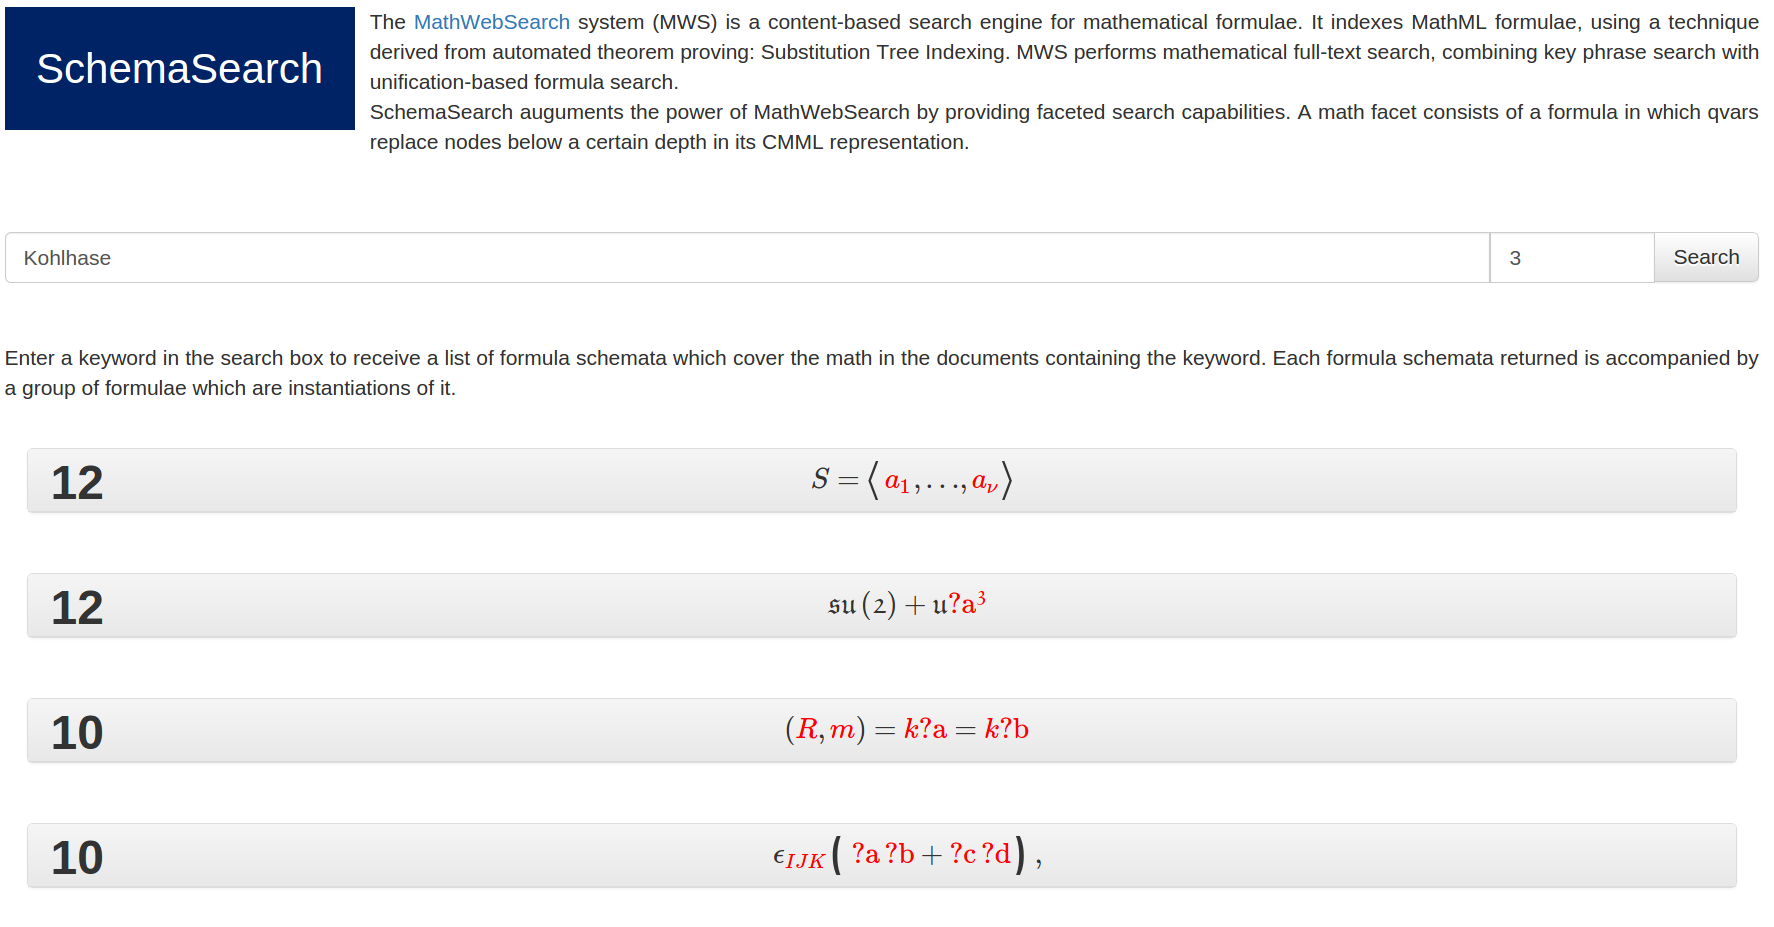
\includegraphics[width=12.1cm]{img/schemataGroup.png}
    \caption{Faceted results at depth 3}\label{fig:schemata_group}
\end{figure}
\FloatBarrier

Figure~\ref{fig:schema_instantiation} shows the expansion of a formula class.
There are $22$ formulae in the class given by this particular math schema, as
indicated by the count on the left upper side, out of which only ten are shown.
We can see $2$ unnamed query variables marked with red as $\red{?a}$ and
$\red{?b}$. By seeing the schema, the user can form an impression about the
general structure of the formulae from that class. After expanding the class,
the listing of concrete formulae appears. If the user clicks on one of them, he
is redirected to the source document from which that expression was extracted.

\begin{figure}[ht]\centering
    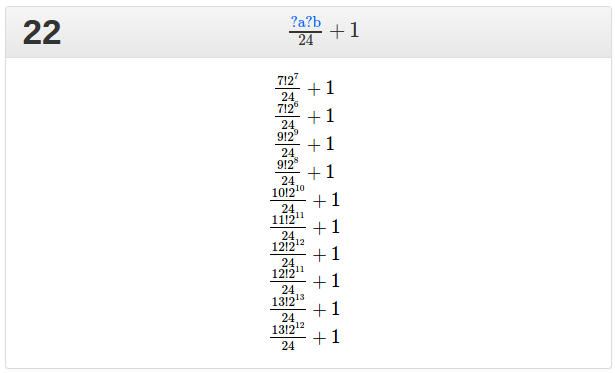
\includegraphics[width=12.1cm]{img/schemaInstGood.png}
    \caption{Expansion of a formula class 1}\label{fig:schema_instantiation}
\end{figure}
\FloatBarrier

Another class expansion which showcases the schematization can be seen in
Figure~\ref{fig:schema_instantiation3}. By seeing this schema, the user can
abstract away the complexity of the formulae and obtain a ``summary'' of the
meaning behind it. Also, by expanding the class he can explore several related
formulae easily, because they are grouped together.
\begin{figure}[ht]\centering
    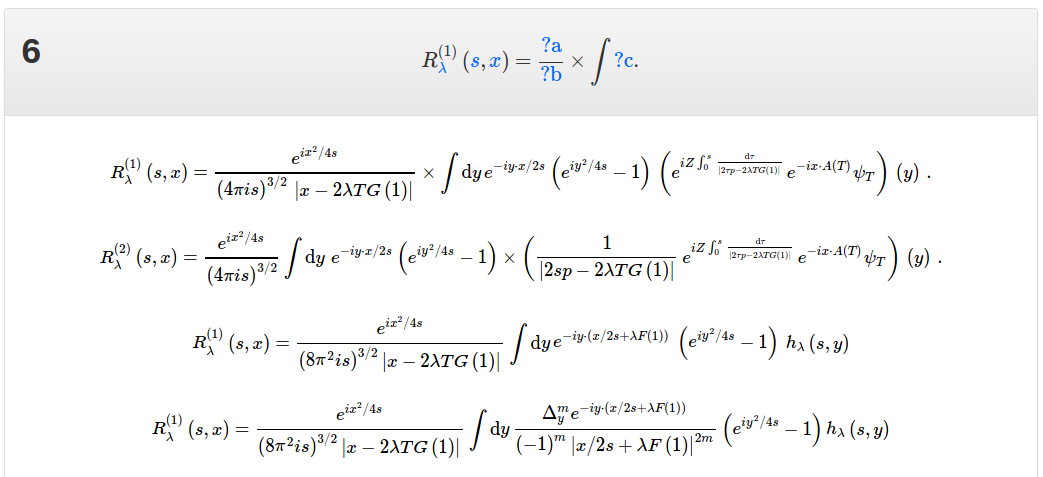
\includegraphics[width=12.1cm]{img/schemaInstGood3.png}
    \caption{Expansion of a formula class 2}\label{fig:schema_instantiation3}
\end{figure}
\FloatBarrier

\subsection{TemaV2 front-end}\label{subsec:fe_results_display2}
Figure~\ref{fig:temaV2_results} shows the results of a query for ``Fermat'' and
${\red{?a}}^{\red{?n}} + {\red{?b}}^{\red{?n}}={\red{?c}}^{\red{?n}}$. Besides
the regular \tms results, the user is also presented with a ``Math Facets''
section.

\begin{figure}[ht]\centering
    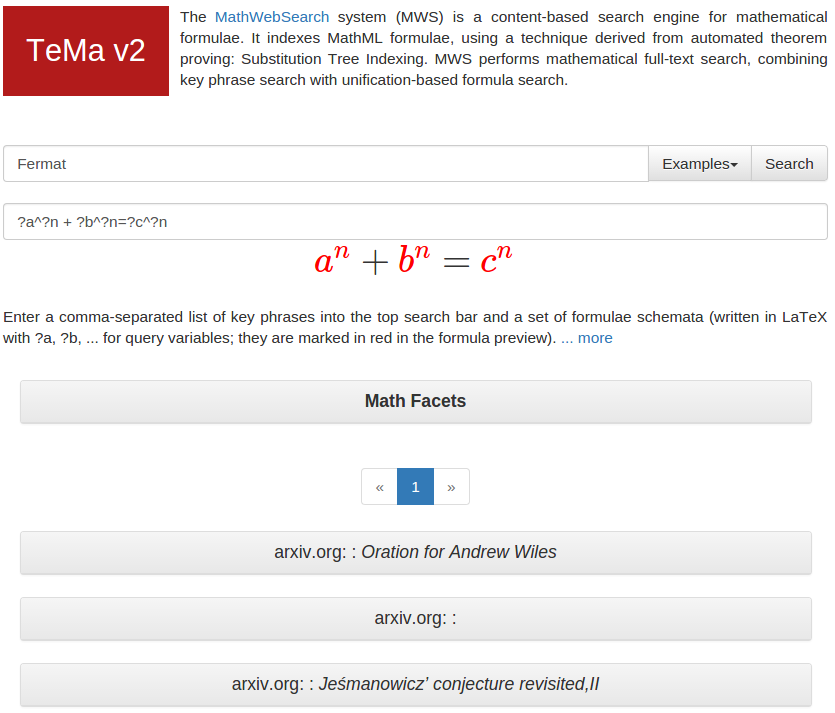
\includegraphics[width=12.1cm]{img/temaV2_results.png}
    \caption{Expansion of a formula class 1}\label{fig:temaV2_results}
\end{figure}
\FloatBarrier

When the ``Math Facets'' section is expanded the user can see the top 10
schemata (ranked with respect to their coverage), as shown in
Figure~\ref{fig:temaV2_facets}. We have also implemented a ``search-on-click''
functionality that allows the user the do a fresh search using the clicked
schema and the initial keyword, which effectively filters the current
results.

\begin{figure}[ht]\centering
    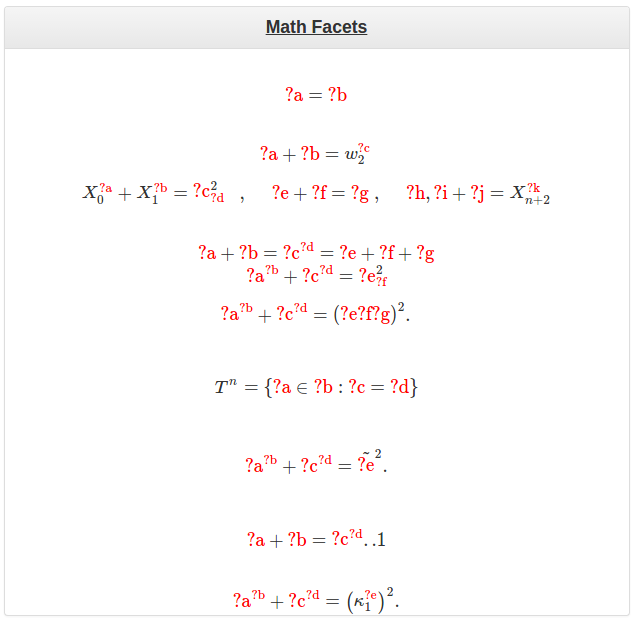
\includegraphics[width=12.1cm]{img/temaV2_facets.png}
    \caption{Expansion of a formula class}\label{fig:temaV2_facets}
\end{figure}
\FloatBarrier


\subsection{Performance of the Schematizer}\label{subsec:sch_performance}
We designed the Schematizer to be a very lightweight daemon, both as memory
requirements and as CPU usage. To test if we achieved this goal, we benchmarked
it on a server running Linux 3.2.0, with 10 cores (Intel Xeon CPU E5-2650
2.00GHz) and 80 GB of RAM. 

We obtained the 1123 expressions to be schematized by querying Elasticsearch by
the keyword ``Fermat''. While the overall time taken by the faceted search
engine was around 5 seconds, less than a second was spent in the Schematizer.
Also, the CPU utilized by the Schematizer never rose higher than 15\% (as
indicated by the \textsf{top} utility). Asymptotically, the algorithm would run
in $O(N)$ time, where $N$ is the number of input formulae. We are able to reach
linear time performance, because each formula is processed exactly once and the
signature is stored in a hash table, as discussed in
Section~\ref{subsec:fschematizer}.

The space complexity is also linear in the number of formulae, because in the
worst case scenario (large cut-off depth) we will have a schema for every
formula. To analyze the memory footprint of the Schematizer we used
Massif~\cite{massif:online}, a heap profiler from Valgrind's tool suite.
Figure~\ref{fig:heap_usage} shows the total heap memory consumption for a
single query (containing 1123 expressions). Massif reports time using the
number of executed instructions as unit of measurement. The heap memory size is
given in bytes.

There is a short initial steep increase moments after the program started.
This can be attributed to the dynamic linker. Then, the consumption keeps
increasing because we are receiving the formulae (storing them in memory) and
generating the schemata. The peak is reached at 20 MiB, which is impressively
low. Afterwards, there is a sudden decrease in heap size when we drop the
schemata which are not needed (because a \textsf{max\_size} parameter was
specified by the caller). For most of the next part, the heap size stays
constant because we are only processing the signatures and finding the PMML
substitution IDs.

\begin{figure}[ht]\centering
    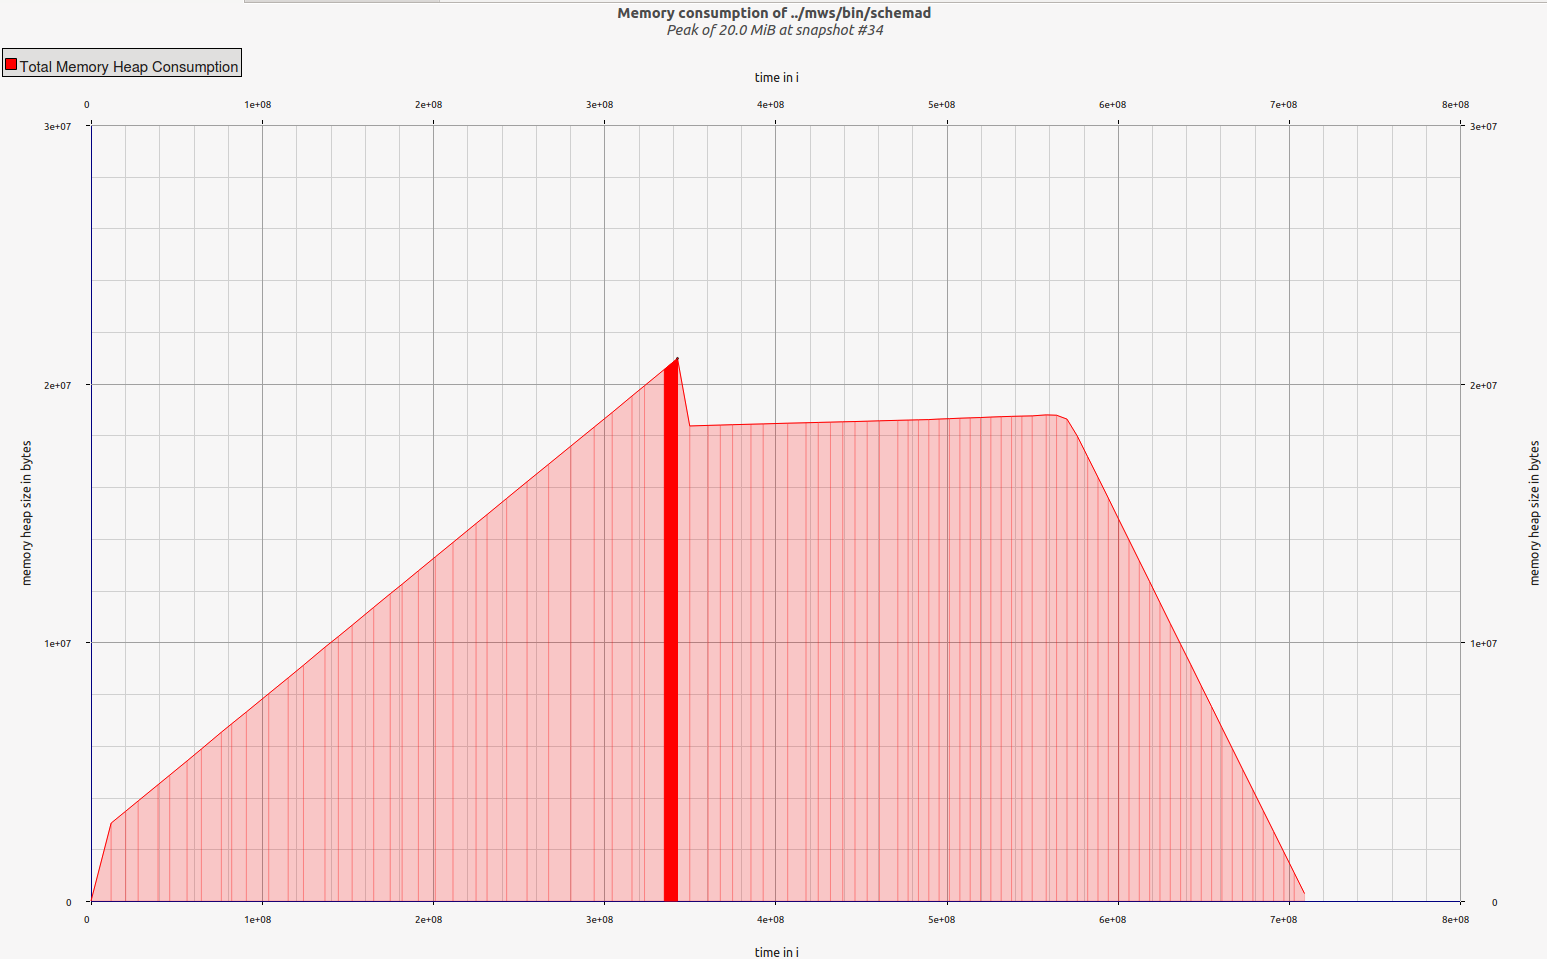
\includegraphics[width=12.1cm]{img/heapUsage.png}
    \caption{Schematizer heap usage for a query}\label{fig:heap_usage}
\end{figure}
\FloatBarrier

All things considered, it is somewhat remarkable that the peak memory usage
is at only 20 MB and only 15\% of one processor is in use for 1123 formulae.
Considering the linear complexity, we can accommodate several millions of
formulae on the mentioned server:
$$80 GB \cdot \frac{1123}{20 MB} \approx 4.5 \cdot {10}^{6} \text{formulae}$$

Due to its implementation, the Schematizer is indefinitely scalable, because it
does not require shared state between formulae and can therefore be implemented
as a MapReduce~\cite{mapreduce} job, where mappers compute the signature of
assigned formulae and reducers assemble the signature hash table.

\subsection{The API}\label{subsec:schematizer_api}
Another relevant point of interest in the Schematizer is its simple, but
sufficient API. By providing an HTTP endpoint, any application which wishes to
use the schematization service can do so, simply by issuing a GET request.
The content of the GET request must be an \xml document, which \verb|mws:query|
as the root element. The children of the \verb|mws:query| are the expressions
to be schematized in \cmml format. The attributes of the query are
\textsf{answsize} (the maximum number of schemata), \textsf{output} (JSON or
XML), \textsf{depth} (the depth for cutoff) and \textsf{cutoff\_mode}
(specifying whether the cutoff should be absolute or relative).  If JSON is
used for the output, the IDs of PMML substitutions will be returned. If XML is
used, formula schemata in CMML format will be returned.

\section{Applications and future work}\label{sec:future}
One improvement angle that can be worked on is the ranking of the schemata.
We have used a simple method, ranking them in decreasing order of coverage,
thus having the schema with most formulae in its class on the first place.
However, this is not always a good approach. When users look at the facets,
it is usually because they were not able to find what they were hoping for
(because the result set is too large). The first schemata cover most of the
formulae users have already looked at, so they are not of interest.
However, the last schemata are not of interest either, because they typically
only cover very rare formulae (1-2 occurrences). A good ranking approach would
place the \textit{medium-coverage} schemata first, then the top-coverage and
then the low-coverage. In order to define precisely what is the range for
medium-coverage, further research is required.

One other application of the faceted search engine can be providing
mathematical definitions with the help of
\textsf{NNexus}~\cite{GinCor:nnexus:14}. NNexus is an auto-linker for
mathematical concepts from several encyclopedias, e.g.  PlanetMath, Wikipedia.
Assuming we are able to generate relevant schemata in response to keyword
queries, we can target the faceted search engine with all the concepts stored
by NNexus and store a schema for each such concept.  Afterwards, for a given
query, we can obtain the schema and check it against our stored set of
schemata. If we find it, we can link the given expression to its mathematical
definition. Given a large number of stored concepts and a high schemata
relevance, the user should be able to see the definition of any encountered
formulae on the web. For example, hovering over $a^2 + b^2 = c^2$ will show the
definition of the Pythagorean theorem.

Another, more direct, application of the Schematizer would be
\textit{Similarity Search}. One could create a \mws based search engine, which
accepts an input formula and a similarity degree (between 0\% and 100\%). The
engine would then create a formula schema at a relative depth corresponding to
the similarity degree and use this schema to search the corpus. This approach
defines the similarity between two formulae as the percentage of the CMML tree
depth that they share.

\section{Conclusion}\label{sec:conclusion}
We have presented the design and implementation of a system capable of faceted
search. Moreover, we have described a general-purpose scalable Schematizer
which can generate recognizable formula schemata and divide expressions into
formula classes according to said schemata. Consequently, we have successfully
addressed all challenges outlined in Section~\ref{subsec:prelim:goals}.

Although the Schematizer provides easily recognizable formulae, some queries on
\schemasearch (e.g. using an author as keyword) provide hits with a very low
relevance. This is because we cannot distinguish between the work of the author
and work where the author is cited at the textual level. As a consequence,
searching for ``Fermat'' would also show formulae from papers where Fermat was
cited and if these papers are numerous, as it happens with known authors, would
provide the user with misleading results. This suggests that a better source of
mathematical expressions might be required for the SchemaSearch demo.

\printbibliography

\end{document}

